\section{System Architecture}
\label{sec:design}

In this section, we describe the design of Themis.

\subsection{Core Architecture}
\label{sec:overview}

Themis reuses several core runtime components that were used to build
TritonSort.  Like TritonSort, Themis is written as a sequence of
\emph{phases}, each of which consists of a directed dataflow graph of
\emph{stages} connected by FIFO queues.  Each stage consists of a number of
\emph{workers}, each running as a separate thread.

\subsection{MapReduce Overview}

\begin{figure*}
\centering
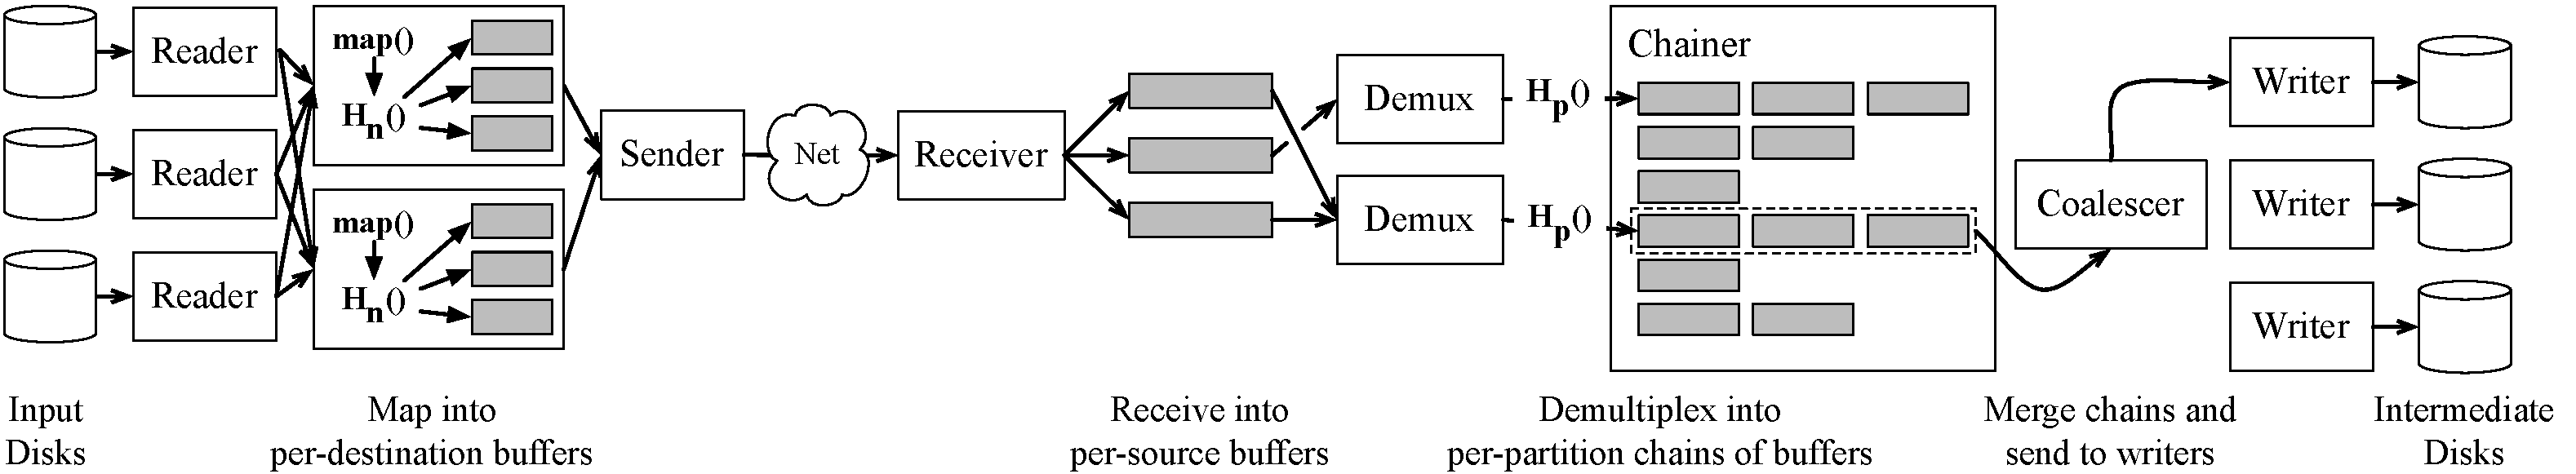
\includegraphics[width=\textwidth]{themis/figures/detailed_phase_one.pdf}
\caption{\label{fig:phase_one} Stages of Phase One (Map/Shuffle) in Themis}
\end{figure*}

Unlike existing MapReduce systems, which executes \map and \reduce tasks
concurrently in waves, Themis implements the MapReduce programming model in
three phases of operation, summarized in Table~\ref{tbl:stages}.  Phase zero,
described in Section~\ref{sec:phase_zero}, is responsible for sampling input
data to determine the distribution of record sizes as well as the distribution
of keys.  These distributions are used by subsequent phases to minimize
partitioning skew.  Phase one, described in Section~\ref{sec:phase_one}, is
responsible for applying the \map function to each input record, and routing
its output to an appropriate partition in the cluster.  This is the equivalent
of existing systems' map and shuffle phases.  Phase two, described in
Section~\ref{sec:phase_two}, is responsible for sorting and applying the
\reduce function to each of the intermediate partitions produced in phase one.
At the end of phase two, the MapReduce job is complete.

\begin{table}
\centering
\caption{\label{tbl:stages} Themis's three stage architecture}
\begin{tabular}{|c|c|c|} \hline
\textbf{Phase} & \textbf{Description} & \textbf{Required?} \\\hline
0 & Skew Mitigation & Optional \\
1 & \texttt{map()} and shuffle & Required \\
2 & sort and \texttt{reduce()} & Required \\\hline
\end{tabular}
\end{table}

Phase one reads each input record and writes each intermediate record exactly
once.  Phase two reads each intermediate partition and writes its corresponding
output partition exactly once.  Thus, Themis has the 2-IO property.

\subsection{Phase One: Map and Shuffle}
\label{sec:phase_one}
\label{sec:map}

Phase one is responsible for implementing both the \map operation as well as
shuffling records to their appropriate intermediate partition.  Each node in
parallel implements the stage graph pipeline shown in
Figure~\ref{fig:phase_one}.

The \Readerbf stage reads records from an input disk and sends them to the
\Mapperbf stage, which applies the \map function to each record.  As the \map
function produces intermediate records, each record's key is hashed to
determine the node to which it should be sent and placed in a
per-destination buffer that is given to the \sender when it is full.  The
\Senderbf sends data to remote nodes using a round-robin loop of short,
non-blocking \texttt{send()} calls.  We call the \Reader to \Sender part of the
pipeline the ``producer-side'' pipeline.

The \Receiverbf stage receives records from remote nodes over TCP using
a round-robin loop of short, non-blocking \texttt{recv()} calls. We implemented
a version of this stage that uses \texttt{select()} to avoid unnecessary
polling, but found that its performance was too unpredictable to reliably
receive all-to-all traffic at 10Gbps. The \receiver places incoming records
into a set of small per-source buffers, and sends those buffers to
the \Demux stage when they become full.

The \Demuxbf stage is responsible for assigning records to partitions.  It
hashes each record's key to determine the partition to which it should be
written, and appends the record to a small per-partition buffer.  When that
buffer becomes full, it is emitted to the \Chainerbf stage, which links buffers
for each partition into separate \emph{chains}.  When chains exceed a
pre-configured length, which we set to 4.5 MB to avoid doing small writes, it
emits them to the \Coalescerbf stage.  The \Coalescerbf stage merges chains
together into a single large buffer that it sends to the \Writerbf stage,
which appends buffers to the appropriate partition file. The combination of the
\Chainer and \Coalescer stages allows buffer memory in front of the \Writer
stage to be allocated to partitions in a highly dynamic and fine-grained way.
We call the \Receiver to \Writer part of the pipeline the ``consumer-side''
pipeline.

A key requirement of the consumer-side pipeline is to perform large, contiguous
writes to disk to minimize seeks and provide high disk bandwidth.  Themis uses
the same node-wide, application-driven disk scheduler used in TritonSort to
ensure that writes are large. We refer the reader to
Section~\ref{sec:tritonsort-disk-scheduler} for details on the disk scheduler's
implementation.

\subsection{Phase Two: Sort and Reduce}
\label{sec:phase_two}
\label{sec:reduce}

\begin{figure}[h]
\centering
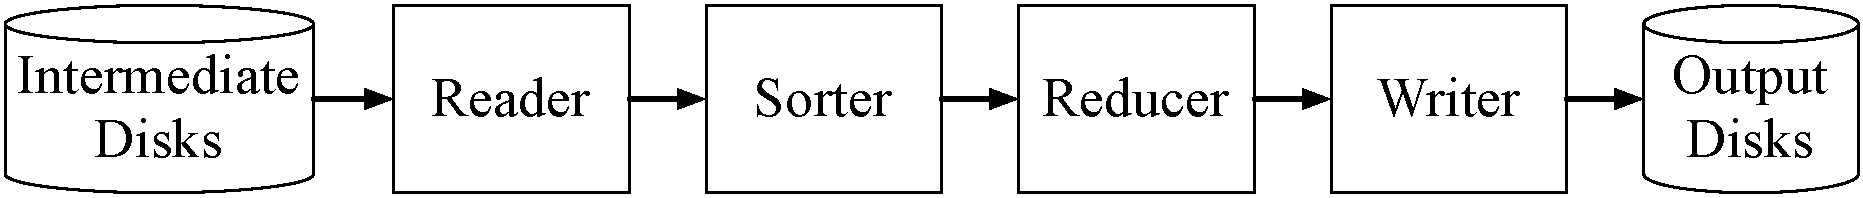
\includegraphics[width=\columnwidth]{themis/figures/phase_two.pdf}
\caption{\label{fig:phase_two} Stages of Phase Two (Sort/Reduce) in Themis}
\end{figure}

By the end of phase one, the map function has been applied to each input
record, and the records have been grouped into partitions and stored on the
appropriate node so that all records with the same key are stored in a single
partition.  In phase two, each partition must be sorted by key, and the \reduce
function must be applied to groups of records with the same key.  The stages
that implement phase two are shown in Figure~\ref{fig:phase_two}.

There is no network communication in phase two, so nodes process their
partitions independently.  Entire partitions are read into memory at once by
the \Readerbf stage. A \Sorterbf stage sorts these partitions by key, keeping
the result in memory.  The \Reducerbf stage applies the \reduce function to all
records sharing a key.  Reduced records are sent to the \Writerbf, which writes
them to disk.

All records with a single key must be stored in the same partition for the
\reduce function to produce correct output. As a result, partitioning skew can
cause some partitions to be significantly larger than others. Themis's memory
management system allows phase two to process partitions that approach the size
of main memory, and its optional skew mitigation phase can reduce partitioning
skew without user intervention. We describe these systems in Sections
\ref{sec:memory} and \ref{sec:phase_zero}, respectively.

A key feature of Themis's \sorter stage is that it can select which sort
algorithm is used to sort a buffer on a buffer-by-buffer basis.  There is a
pluggable \textit{sort strategy} interface that lets developers use different
sorting algorithms; currently quicksort and radix sort are implemented.  Each
sort strategy calculates the amount of scratch space it needs to sort the given
buffer, depending on the buffer's contents and the sort algorithm's space
complexity.  For both quicksort and radix sort, this computation is
deterministic.  In Themis, radix sort is chosen if the keys are all the same
size and the required scratch space is under a configurable threshold;
otherwise, quicksort is used.
